\chapter{Increment one}
\label{chap:Increment one}
In this chapter the group will go through the requirements of the project and explain how these requirements can and has been implemented. The result of this would be a new set of requirements with some of the same requirements, new requirements and changed requirements.  

\section{Requirements}
\label{sec:i1Requirements}
The requirements considered in this increment are marked with blue colouring.

\begin{itemize}
	\item When a user throws an object towards the trash bin, within the predefined area, the bin should always catch the object
	\begin{itemize}
		\item \textcolor{blue}{The robots predefined area should be calculated from the hardware limitations of the motors’ speed}
	\end{itemize}
	\item The robot should know where it is positioned
	\begin{itemize}
		\item \textcolor{blue}{The robot should have a starting position, from where it should be able to calculate it's current position }
		\item \textcolor{blue}{The robot's starting point should be placed outside its predefined area, such that it moves forward into the area}
	\end{itemize}
	\item The robot should be able to detect and track the thrown object
	\begin{itemize}
		\item \textcolor{blue}{The thrown object should be detected and tracked by a Microsoft Kinect}
		\item The Kinect should send the coordinates of the impact point of the object to the robot
	\end{itemize}
	\item The robot should be able to calculate the impact point for the object
	\begin{itemize}
		\item \textcolor{blue}{Trajectory prediction should be used to calculate the impact point of the thrown object}
	\end{itemize}
	\item The robot should be able to move the trash bin, such that the thrown object lands inside the bin
	\begin{itemize}
		\item \textcolor{blue}{The robot should be able to turn and drive forward and backwards}
		\item {The robot should be able to recognize the coordinates sent from the Kinect}
	\end{itemize}
	\item {The robot should be able to receive data from a computer, through a wireless network}
	\item {The system tasks should be able to be scheduled and verified}
\end{itemize}

These requirements are rudimentary, and the very essence of the project lies within the fulfilment of these requirements. In this increment the fundamentals of the robots movement should be implemented, the predefined area should be defined, a starting point for this area should be determined and the Microsoft Kinect should be able to detect and track an object by using trajectory prediction.

\section{System design}
\label{sec:i1System Design}
The following sections describe how the marked requirements in \ref{sec:i1Requirements} should be fulfilled. The theories and ideas will be explained subsequently.

\subsection{Predefined area}
\label{sec:i1Predefined area}
The robots predefined area, is an area where the robot should catch the object within. This area is being made because of the limitations of the robots motors and is based on motor speed and average time of a throw, so the predefined area is where the robot should be expected to catch the object within.

\subsection{Throwing}
\label{sec:i1Throwing}
The reason why the throw of the object (which in this project will be a table tennis ball) is important, is because the robot should have as much time to move to the collision point as possible. Before the robot moves to the collision point, the Kinect should calculate the where the robot should move, send the data to the robot, and the robot then moves. The Kinect can at any point send new data to the robot, so its course have to be changed, therefore it is important for the robot to have sufficient time to move within the predefined area.    

\subsection{Microsoft Kinect}
\label{sec:i1Microsoft Kinect}
To detect the object, the Kinect has to use one of its cameras, more specifically the depth sensor. The depth sensor uses a range of infrared speckles that draw a pattern in the room. Every cluster of speckles can be identified from each other, which makes the Kinect able to differentiate between objects in the room. The depth of the specific object can be determined by the use of two cameras, as both cameras can identify the speckles at the object and then triangulate the distance between the cameras and the object. This speckle pattern technology will only work indoor, and limits the use to only one kinect, as the speckles can be washed out by other lightsources.
\citep{kw}

\subsection{Trajectory prediction}
\label{sec:Trajectory prediction}
When the object, referred to in this section as the projectile, is detected and the tracking of that projectile has started, the trajectory can be predicted. This prediction is limited to the amount of data sent by the sensory camera, meaning that for every camera reading, one detection of the object is gained. The precision of the prediction will increase according to the time a projectile has been tracked. \newline 
In this project the outdoor weather conditions, that might affect the projectile trajectory, are not considered,  since the prediction is done indoor. As well, the effects of air resistance, also called drag, will not be considered.

The trajectory of a projectile is the path of a thrown projectile affected by gravity, without propulsion. To calculate a trajectory of a projectile, the initial height, the angle which the projectile is launced from, the speed of the projectile at launch and the gravitational acceleration must be taken into account. \newline 
The initial height in this project is the height at which the projectile is detected. The angle and speed at which the projectile is launched, will be calculated from the first few trackings after detecting the projectile. The gravitational acceleration is considered as \(9.81m/s^2\), which is the common value near the earths surface. \newline

To catch the projectile, the distance and time of flight have to be calculated. This is done with two mathematical formulas:
\newline 
\begin{math}
g: \ the \ gravitational \ acceleration \ (9.81m/s^2)\newline
\theta: \ the \ angle \ at \ launch 
v: \ the \ speed \ at \ launch\newline
y_{0}: \ the \ initial \ height\newline
d: \ the \ total \ horizontal \ distance \ traveled \ \newline
t: \ the \ time \ of \ flight\newline
v_{vert}: \ the \ vertical \ velocity\newline
v_{hori}: \ the \ horizontal \ velocity\newline
t_{h}: \ the \ time \ since \ first \ detection\newline
d_{t}: \ the \ distance \ at \ time \ t\newline
\end{math}

The above variables can express the formulas needed to provide the total distance traveled by the projectile, and the time of flight.\newline

Distance traveled:
\[d = \dfrac{v \ cos \ \theta}{g}(v \ sin \ \theta + \sqrt{(v \ sin \ \theta)^2 \ + \ 2gy_{0}})\] \newline
Time of flight:
\[t = \dfrac{d}{v \ cos \ \theta} = \dfrac{v \ sin \ \theta \ + \ \sqrt{(v \ sin \ \theta)^2 \ + \ 2gy_{0}}}{g}\]
\newline

To predict the trajectory of the projectile, the altitude and distance of the projectile at any time during the flight must be calculated, according to the initial height ( \(y_{0}\) ):
\[y = v_{vert}t - \dfrac{1}{2} gt^2\]
\[d_{t} = v_{hori}t\]

After this section, the projectile can be tracked, and the path for a given projectile can be calculated to a certain degree of precision. 

\subsection{Gyroscope and Accelerometer}
\label{sec:i1Gyroscope and Accelerometer}
For positioning the robot, the Lego NXT Gyro and Accelerometer sensors will be considered. These sensors will be used together to position the robot, as the gyroscope will tell the number of degrees the robot has turned, which is relative to the heading of the robot at the first recording of data. This heading will be used together with an accelerometer, which can be used to calculate the distance the robot has traveled since the first recording of data. The speed, travel time and heading will be the data of these sensors.


\subsection{Movement}
\label{sec:i1Movement}
The robot is expected to be able to drive both forward and backwards. The robot is expected to turn using either one active wheel, or using both wheels in a counterclockwise motion in order to turn faster.


\section{Implementation}
\label{sec:i1Implementation}
This section explains how the marked requirements has been implemented and whether or not the group changed the requirement, as something didn't work out as expected. 

\subsection{Gyroscope and Accelerometer in use}
\label{sec:i1Gyroscope and Accelerometer in use}
For the implementation of the gyroscope and the accelerometer, a test has to be done, to benchmark the precision of the sensors. For this, the data sent from the Arduino when the sensor has been plugged into the Arduino, was plotted in the Serial Plotter, which is a feature in the Arduino IDE. 

The accelerometer would not be precise enough to calculate the distance the robot had moved. The accelerometer would give an acceleration, to calculate from an acceleration to a distance, the time had to be multiplied to the acceleration twice. If the acceleration was not precise, this would lead to a big margin of error. 

The gyroscope worked just fine, but when it was not moving, the data seen in the Serial plotter would wander. This meant that when reading data from the gyroscope, either the gyroscope should be reset before reading data or the value would be the difference of when it started reading till it stopped. 

Instead of using the gyroscope and the accelerometer, it was decided to use the motor' encoderes, which can be used to calculate the heading and the distance moved. 


\subsection{Predefined area}
\label{sec:i1Predefined areaImplementation}
The robots predefined area will be calculated using the time of flight and the speed of the motors. 
This predefined area is limited to be strictly in front of the robot.
A bouncing throw would have a travel time of 2 - 2.15 seconds, explained in greater detail in section \ref{sec:i1ThrowingImplementation}. The predefined area was constructed using the robot itself. The robot was placed marking its starting point, and was set to turn a specific number of degrees and move forward for two seconds. After a series of runs, the area marked by the robot turned out as shown in figure \ref{figure:Predefined area}. The predefined area measures 2851.5cm\begin{math}^2\end{math}.

\begin{figure}[h]
\centering
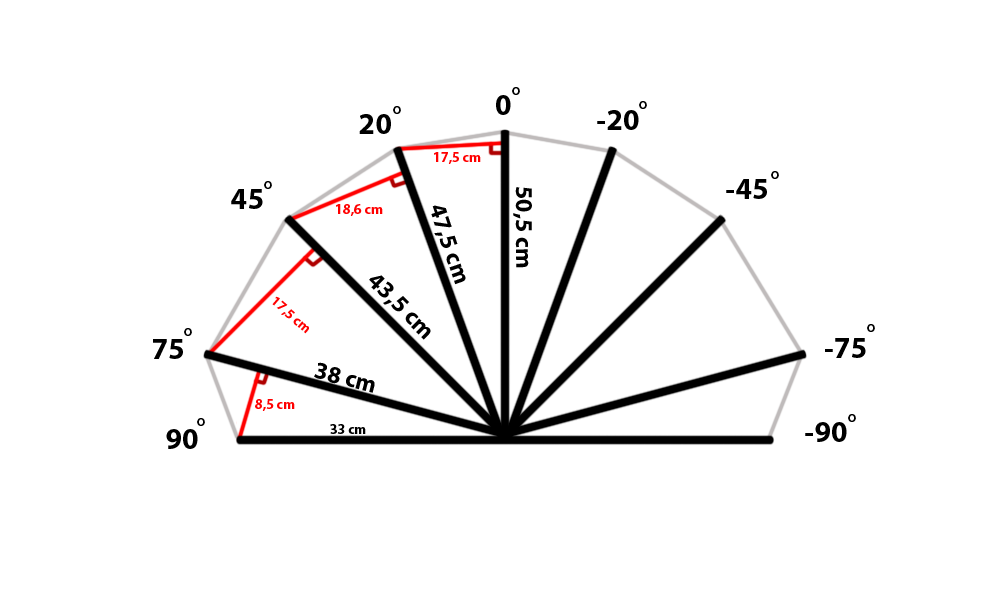
\includegraphics[scale=0.35]{billeder/predefined-area}
\caption{The robots predefined area}
\label{figure:Predefined area}
\end{figure}

\subsection{Throwing}
\label{sec:i1ThrowingImplementation} 
To ensure that the robot is provided the maximum amount of time for calculations and movement, the average time of flight of an object at a designated distance was measured. At a distance of three meters, the average time of flight of the object was 1.1 seconds, and at a distance of five meters, the average time of flight was 1.25 seconds.

With the results from the abovementioned measurements, it is concluded that a regular throw would not provide enough time for the robot to catch the object. As mentioned in the \ref{sec:LEGO NXT Servo motor} section, the robots speed was calculated to be ~87 RPM. With a 1.1 seconds time of flight, with a distance of three meters, the impact point should be within a 280 mm radius from the robot. This simply is not fast enough to catch the object from a three or five meter distance.

This introduces the idea of bouncing the object, in order to solve the above mentioned problem. The idea is, that the initial height of the object is considered to be the floor instead of the top half of the arc, which in theory should provide more time for the robot. \newline
After conducting another set of tests, this theory proved to be correct. The average time of flight at a distance of three meters is 2 seconds, and at a distance of five meters the average time of flight is on average 2.15 seconds. The bouncing throw provides the robot with close to double the amount of time.

\subsection{Microsoft Kinect}
\label{sec:i1Microsoft KinectImplementation}

\subsection{Movement}
\label{sec:i1MovementImplementation}
An Arduino Motor Shield is used to enable greater control of the movement of the motors through the motor shields library called Adafruit which is included through \#include <AFMotor.h> (unsure how to present this nicely)
The Arduino Motor Shield and library enables manipulation of the individual wheels instead of only being able to either rotate forward or backwards on both wheels simultaneously. 
The wheels were tested and forward motion was achieved with a speed of roughly 25.5 centimetres per second. It was discovered that the speed at which the robot drives backwards is much slower than its forward moving speed, because of the speed of backwards motion, it was decided to not consider driving backwards at all since the speed were inadequate and since this would also simplify the problem, and could later be solved with different motors. To solve this issue, it was decided to change the throw to always be in front of the machine, thus ensuring it would never be forced to drive backwards. This does however not take into account if the Kinect projectile prediction predicts the projectile will land behind the machine but this issue only arises if prediction is sufficiently miscalculated which is unlikely.

\section{Evaluation}
\label{sec:i1Evaluation}
This section will include a short summary of the chapter, ending up with a new requirement list, based on the how the group implemented the marked requirements from the beginning of the chapter.


The requirements stating that the robot should know where it is positioned, will persist through this increment, as no solution was found in this increment. The use of a gyroscope and accelerometer was not the right solution for this project, as the need of precise data would not be supported by sensors with a large amount of jitter. Another way of positioning the robot would be by calculating the distance traveled on each wheel, through the motor encoder in the NXT servo motors. The distance traveled would be calculated by the rotation of the wheel and the circumference of that wheel.
The robots starting position will always determine where the predefined area of the robot is along with its hardware limitations. The concept of a predefined area is entirely based on the rotation speed of each motor, the wheel circumference and the duration of the throw. If any element that defines the predefined area changes, then so does the predefined area. Movement was not nearly as simple as expected and the implications of the problems encountered in its implementation is not fully solved in this increment.

The requirement of driving forward and backwards is redefined as only consisting of driving fowards. The reason for the change was explained in the section \ref{sec:i1Movement}.

The requirements after finalizing increment one is:
\begin{itemize}
\item The trash bin should catch the trash if the user throws it towards the trash bin and within a predefined area
\begin{itemize}
	\item \textcolor{green}{The robots predefined area should be calculated from the hardware limitations of the motors’ speed}
\end{itemize}
\item The robot should know where it is positioned
\begin{itemize}
	\item \textcolor{red}{The robot should have a starting position, from where it should be able to calculate it's current position through calculations of the motor encoders}
	\item \textcolor{green}{The robot's starting point should be placed outside its predefined area, such that it moves forward into the area}
\end{itemize}
\item The robot should be able to detect and track the thrown trash
\begin{itemize}
	\item \textcolor{green}{The thrown trash should be detected and tracked by a Microsoft Kinect}
	\item The Kinect should send the coordinates of the impact point of the trash to the robot
\end{itemize}
\item The robot should know where the the thrown trash will land
\begin{itemize}
	\item \textcolor{green}{Trajectory prediction should be used to calculate impact point of the thrown trash}
\end{itemize}
\item The robot should be able to move the trash bin, such that the thrown trash lands inside the bin
\begin{itemize}
	\item \textcolor{orange}{The robot should be able to turn and drive forward}
	\item {The robot should be able to recognize the coordinates sent from the Kinect}
\end{itemize}
\item {The robot should be able to receive data from a computer, through a wireless network}
\item {The system tasks should be able to be scheduled and verified}
\end{itemize}
